\documentclass[UTF8]{ctexart}
\usepackage[table]{xcolor}
\usepackage{algorithm}
\usepackage{algorithmic}
\usepackage{subfigure}
\usepackage{amsmath,bm}
\usepackage{fancybox}
\usepackage{listings}
\usepackage{xcolor}
\usepackage{diagbox}
\usepackage{amssymb}
\usepackage{amsmath}
\usepackage{amsthm}
\usepackage{empheq}
\usepackage{warpcol}
\usepackage{lscape}
\usepackage[framemethod=tikz]{mdframed}
\usepackage{mathtools}
\usepackage{fancyhdr} 
\usepackage{longtable,booktabs}                               
\usepackage{lastpage}                                           
\usepackage{layout} 


% 图表
\usepackage{array,multirow}
  \setlength\extrarowheight{2pt} % 行高增加
\usepackage{longtable}
\usepackage{graphicx}

\usepackage{listings}

\usepackage{xcolor}

	\definecolor{ocre}{RGB}{243,102,25}
	\definecolor{mygray}{RGB}{243,243,244}

%
%\lstset{
%columns=flexible,
%numbers=left,
%numberstyle=\footnotesize\color{darkgray}, 
%basicstyle=\small\ttfamily,
%stringstyle=\color{purple},
%keywordstyle=\color[RGB]{40,40,255}\bfseries,
%commentstyle=\it\color[RGB]{0,96,96},  
%stringstyle=\rmfamily\slshape\color[RGB]{128,0,0}, 
%showstringspaces=false,      
%% directivestyle=\color{blue},
%frame=shadowbox,
%%framerule=0pt,
%backgroundcolor=\color[RGB]{245,245,244},
%escapeinside=``, %逃逸字符(1左面的键),用于显示中文
%breaklines,
%extendedchars=false,
%%解决代码跨页时,章节标题,页眉等汉字不显示的问题
%xleftmargin=2em,xrightmargin=2em,
%aboveskip=1em,%设置边距
%tabsize=4, %设置tab空格数  
%showspaces=false %不显示空格 
%rulesepcolor=\color{red!20!green!20!blue!20}
%%rulesepcolor=\color{brown}
%}



% 行号
\usepackage{lineno}


% 引用
\usepackage[colorlinks=true,
            pdfborder=001,     
            citecolor=blue,
            linkcolor=red,
            anchorcolor=green,
            urlcolor=blue,
            bookmarksopen=true,bookmarksnumbered=true]{hyperref}
\usepackage{framed} 
\usepackage{ulem}
\usepackage{tabu}
\title{\heiti 稀疏自编码神经网络}
\author{张晋}
\begin{document}
\maketitle
\section{Introduction}
监督学习是人工智能最强大的工具之一,在自动压缩编码识别,语音识别,自动驾驶等方面都取得了重大成就,然而其学习过程仍然要求我们手动指定给算法的输入特征$x$,如果我们给出了一个
好的特征表示,那么这个监督学习算法就可以做得很好,
但是手动标记特征是一个很慢的方法,因而其学习过程受到了极大限制。

因此,我们希望有一种算法能够自动学习比手动设计更好的特征表示,那就是稀疏自动编码器学习算法,这是从未标记数据自动学习特征的一种方法。


\section{Autoencoders and sparsity}
\subsection{自编码器}
自编码器可以理解为一个试图去还原其原始输入的系统。如下图所示。
\begin{figure}[H]
\centering
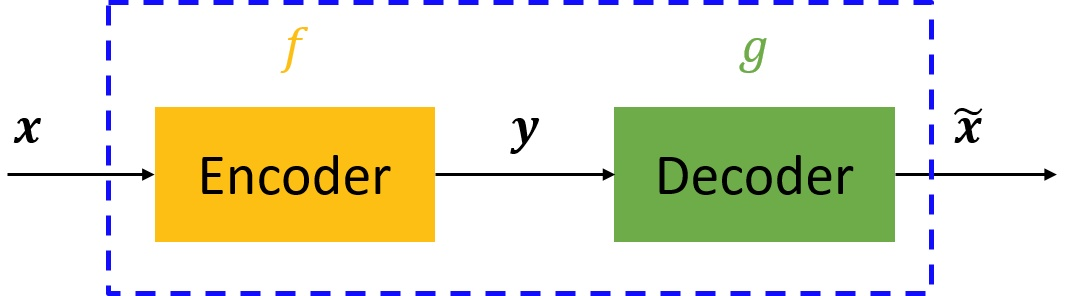
\includegraphics[width=8cm]{fig/s1.jpg}
\end{figure}

虚线蓝色框内就是一个自编码器模型,它由编码器(Encoder)和解码器(Decoder)两部分组成,编码器将输入信号$x$通过$f$变换成编码信号$y=(x)$,而解码器将编码信号$y$通过$g$转换成输出信号$\tilde{x}=g(y)=g(f(x))$

而自编码器的目的是,让输出$\tilde{x}$尽可能复现输入$x$,然而如果$f$和$g$都是恒等映射,那不就恒有$\tilde{x}=x$了吗,因此,我们经常对中间信号y(也叫作“编码”)做一定的约束,这样,系统往往能学出很有趣的编码变换$f$和编码$y$


\subsection{自编码神经网络}
我们可以通过一个三层的神经网络来完成一个自编码器,它使用了反向传播算法来使让目标值等于输入值\footnote{注意自编码神经网络是一个无监督学习算法,因此训练集$\{x^{(1)}, x^{(2)}, x^{(3)}, \ldots, x^{(m)}\big|x^{(i)} \in \Re^{n}\}$ 是没有带标签的.},比如 $ y^{(i)} = x^{(i)} $。

注意,其输出层的神经元个数与输入层是相等的,常用激活函数有:sigmoid、tanh、max($x,0$).下图是一个自编码神经网络的示例。


\begin{figure}[H]
\centering
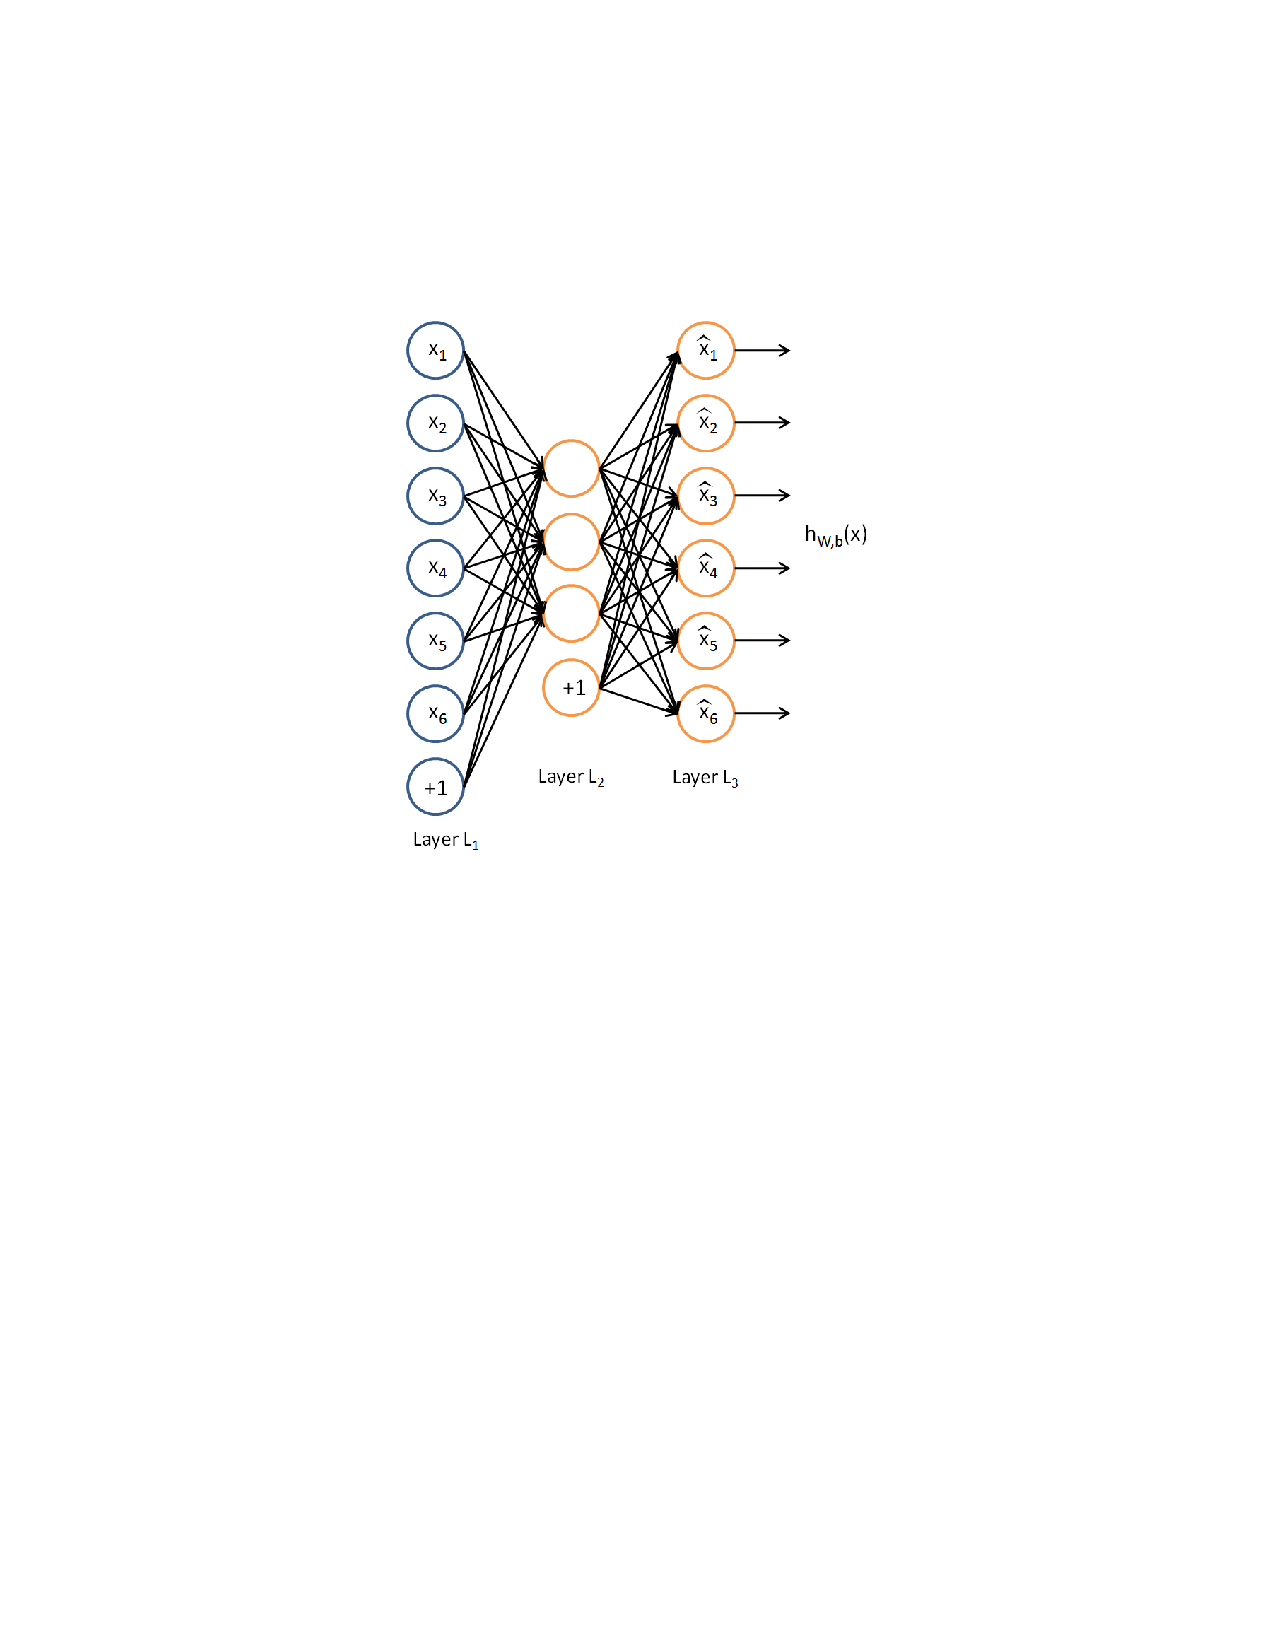
\includegraphics[width=8cm]{fig/1_1.pdf}
\end{figure}


自编码神经网络尝试学习一个 $ h_{W,b}(x) \approx x $的函数,也就是恒等函数,从而使得输出 $ \hat{x} $接近于输入 $ x$ 。

\subsection{自编码神经网络的作用}
有人可能会有疑惑,学习这样一个恒等函数有什么用呢?

这就要谈到压缩编码,一般来说,我们的输入$ x^{(1)}, x^{(2)}, x^{(3)}, \ldots, x^{(m)}$之间是有内在联系的,从信息论的角度来说,就是我们能找到一种更简洁的编码形式来表示它们。

在Hinton的论文\emph{Learning Intemal Representations
by Error Propagation}中,就举出了这样一个例子:构建一个神经网络将以下N位的单位向量映射到本身。
\begin{table}[!tbh]
\caption{\quad 编码问题}
\centering
\begin{tabular}{c c c}  \hline
\qquad 输入\,\,\,\,\,\,\,\,\,\,\,\, &	&\qquad 输出\,\,\,\,\,\,\,\,\,\,\,\, \\ \hline
10000000&$\rightarrow$&10000000\\
01000000&$\rightarrow$&01000000\\
00100000&$\rightarrow$&00010000\\
00010000&$\rightarrow$&00010000\\
00001000&$\rightarrow$&00001000\\
00000100&$\rightarrow$&00000100\\
00000010&$\rightarrow$&00000010\\
00000001&$\rightarrow$&00000001\\\hline
\end{tabular}
\label{Tcode1}
\end{table}



从这个输入中,我们可以发现这是一串二进制数字,尽管位数很长,每个输入$x^{(i)}$占了8bit,但信息量却很低,用信息熵公式
\[\mathrm{H} (X)=-\sum _{{i}}{{\mathrm  {P}}(x_{i})\log _{2}{\mathrm  {P}}(x_{i})}\]

可以算得每个输入$x^{(i)}$蕴含的信息为3/8bit,从而整个样本集蕴含的信息量为3bit,那么从理论上来说,我们就可以把它的信息压缩,从8位压缩到3位。

对应到神经网络上,就是设置8个输入神经元,3个隐藏神经元,从输入神经元到隐藏神经元,这是压缩编码的过程;再设置8个输出神经元,从隐藏神经元到输出神经元,对应的就是解码过程。

\begin{figure}[H]
\centering
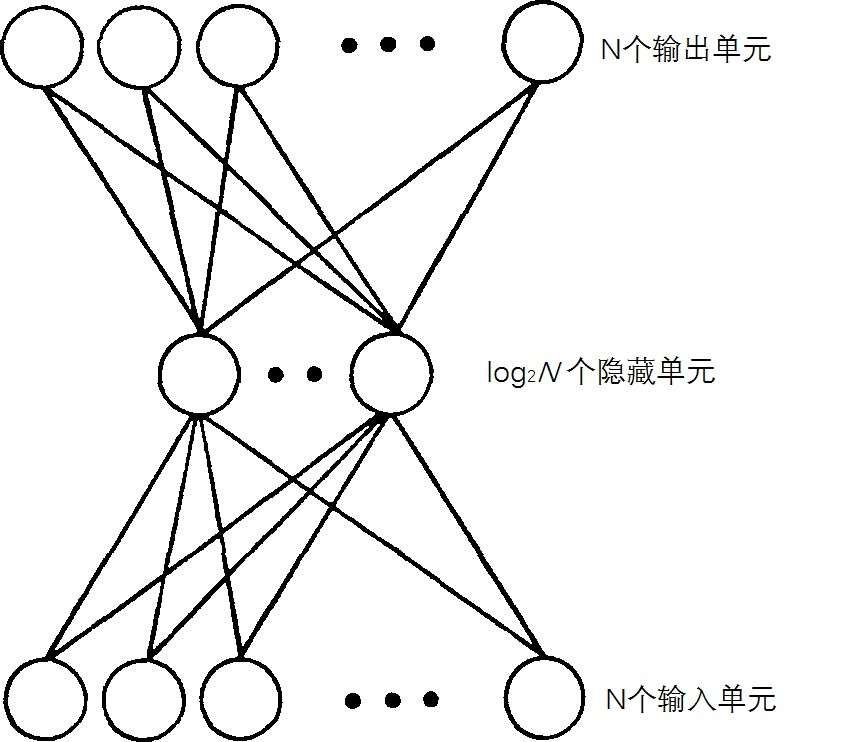
\includegraphics[width=6cm]{fig/s2.png}
\caption{解决该问题的神经网络的基本架构}
\end{figure}

现在我们来设置神经网络的参数:
学习率$\eta=1$,动量学习率$\mu=0.8$,最大迭代次数$maxcount=100000$,终止精度$eps=10e-4$\footnote{程序中的损失函数定义为交叉熵函数,而最后输出的为均方误差值},minibatch的$size=7$,运行\verb|Encode_test.m|程序,运行结果如下:

\small
\begin{verbatim}
Cost =
   4.2151e-07
   
L(3).a =
0.9994   0.0001   0.0000   0.0003   0.0000   0.0000   0.0000   0.0001
0.0002   0.9997   0.0002   0.0000   0.0000   0.0001   0.0000   0.0000
0.0000   0.0002   0.9996   0.0001   0.0000   0.0000   0.0001   0.0000
0.0002   0.0000   0.0002   0.9994   0.0002   0.0000   0.0000   0.0000
0.0000   0.0000   0.0000   0.0002   0.9996   0.0000   0.0001   0.0002
0.0000   0.0002   0.0000   0.0000   0.0000   0.9994   0.0003   0.0003
0.0000   0.0000   0.0002   0.0000   0.0002   0.0000   0.9997   0.0000
0.0004   0.0000   0.0000   0.0000   0.0002   0.0001   0.0000   0.9994

L(2).a =
0.0013   0.0020   0.0023   0.2154   0.9972   0.9993   0.9235   0.7239
0.0028   0.9874   0.9979   0.0835   0.0034   0.9976   0.9912   0.0025
0.6127   0.9988   0.1309   0.0008   0.2528   0.9943   0.0017   0.9991

The corresponding binary:
  001      011      010      000      100      111      110      101
\end{verbatim}
\normalsize

可以发现,我们的神经网络完美地完成了自编码的过程,并且观察隐藏神经元的激活值,可以看出神经网络将每一个输入都匹配了不同的二进制编码,如果只保留前面两层的数据,那么我们就得到了一个压缩函数$f(x)$.

在以上例子中,我们限制了隐藏神经元的个数\textbf{小于}输入神经元的个数,这就迫使自编码神经网络去学习输入数据的压缩表示,网络试图以更小的维度去描述原始数据而尽量不损失数据信息,因为它还必须要能从压缩表示中\textbf{重构}出原来的输入。

这种编码维度小于输入维度的自编码器称为\textbf{欠完备(undercomplete)}自编码器。
由于被迫的降维,欠完备自编码器会自动习得训练样本最显著的特征(变化最大,信息量最多的维度)。\footnote{当编码器是线性,误差函数为二次函数时,欠完备自编码器会学习出与PCA相同的生成子空间,即主元子空间;而当编码器非线性时,它能学到更强大的PCA非线性推广。}

\subsection{稀疏自编码器}
我们知道,编码维度小于输入维度时,自编码器可以训练数据中最显著的特征,但是,当隐藏编码的维数与输入相等,甚至大于输入的\textbf{过完备(overcomplete)}情况下,可能会出现$f,g$都是恒定函数的情况,或者$f(x)=x+1,g(x)=x-1$的情况,这样即使自编码器能使输出 $ \hat{x} $接近于输入 $ x$ ,也不能学到任何有用的信息。

这时,我们需要对自编码器加入一些限制条件来发现输入数据中的结构,比如\textbf{稀疏性限制},这将迫使系统不得不在大量维度中找出真正重要的维度。

\textbf{稀疏性}可以被简单地解释如下:当神经元的输出接近于1的时候我们认为它被激活,而输出接近于0的时候认为它被抑制,那么使得神经元大部分的时间都是被抑制的限制则被称作稀疏性限制。\footnote{这里我们假设的神经元的激活函数是sigmoid函数。如果使用tanh作为激活函数的话,当神经元输出为-1的时候,我们认为神经元是被抑制的.}


我们用 $ a^{(2)}_j(x) $来表示在给定输入样本为$ x $情况下,自编码神经网络隐藏神经元 $ j $的激活值,让
\begin{align}
\hat\rho_j = \frac{1}{m} \sum_{i=1}^m \left[ a^{(2)}_j(x^{(i)}) \right]
\nonumber \end{align}
表示隐藏神经元 $ j $的平均激活值(在训练集上取平均)。

我们加入稀疏性限制:令$\hat\rho_j = \rho$。
其中, $ \rho $是\textbf{稀疏性参数},我们理想中$\rho $
最好是趋于0的,但这在现实中不可能达到(就算达到了,也等于什么都没学到)。所以我们退而求其次,让$ \rho $是一个接近于0的较小的值(比如 $ \rho = 0.05 $)。

为了实现这一限制,我们在目标函数中加入一个罚函数:
\begin{align}
\sum_{j=1}^{s_2} {\rm KL}(\rho || \hat\rho_j)=\sum_{j=1}^{s_2} \rho \log \frac{\rho}{\hat\rho_j} + (1-\rho) \log \frac{1-\rho}{1-\hat\rho_j}.
\nonumber \end{align}
这里, $ s_2 $是隐藏层中隐藏神经元的数量,而索引 $ j $依次代表隐藏层中的每一个神经元。

 现在,我们的总体代价函数可以表示为
\begin{align}
J_{\rm sparse}(W,b) = J(W,b) + \beta \sum_{j=1}^{s_2} {\rm KL}(\rho || \hat\rho_j),
\nonumber \end{align}


其中 $ J(W,b) $ 如之前所定义,而 $ \beta $ 控制稀疏性惩罚因子的权重。 $ \hat\rho_j $ 项则也(间接地)取决于 $ W,b$  ,因为它是隐藏神经元 $ j $ 的平均激活值,而隐藏层神经元的激活值取决于 $ W,b $ 。

\subsection{计算}
在给代价函数增添了罚函数后,我们需要对原BP算法进行改动,我们记
$\qquad B=\beta \sum_{j=1}^{s_2} {\rm KL}(\rho || \hat\rho_j),\qquad J_{\rm sparse}(W,b)=J+B.$
\begin{align}
\delta^{(3)}_i &= \dfrac{\partial J_{\rm sparse}(W,b) }{\partial z_i^{(3)}}\nonumber\\
&=\dfrac{\partial J(W,b) }{\partial z_i^{(3)}}+\dfrac{\partial B }{\partial z_i^{(3)}}\nonumber\\
&=\dfrac{\partial J(W,b) }{\partial z_i^{(3)}}\nonumber \\
\delta^{(2)}_i &= \dfrac{\partial J_{\rm sparse}(W,b) }{\partial z_i^{(2)}}\nonumber\\
&=\dfrac{\partial J(W,b) }{\partial z_i^{(2)}}+\dfrac{\partial B }{\partial z_i^{(2)}}\nonumber\\
&=\dfrac{\partial J(W,b) }{\partial z_i^{(2)}}+
\dfrac{\partial B }{\partial \hat\rho_i}
\dfrac{\partial \hat\rho_i }{\partial a_i^{(2)}}
\dfrac{\partial a_i^{(2)} }{\partial z_i^{(2)}}\nonumber\\
&=
 \dfrac{\partial J(W,b) }{\partial z_i^{(2)}}
+ \beta \left( - \frac{\rho}{\hat\rho_i} + \frac{1-\rho}{1-\hat\rho_i} \right) f'(z^{(2)}_i) 
\nonumber\end{align}

在原BP算法中,我们已经计算了
\begin{align}
\delta^{(2)}_i = \left( \sum_{j=1}^{s_{2}} W^{(2)}_{ji} \delta^{(3)}_j \right) f'(z^{(2)}_i),
\nonumber \end{align}

现在我们只需将其换成
\begin{align}
\delta^{(2)}_i =
  \left( \left( \sum_{j=1}^{s_{2}} W^{(2)}_{ji} \delta^{(3)}_j \right)
+ \beta \left( - \frac{\rho}{\hat\rho_i} + \frac{1-\rho}{1-\hat\rho_i} \right) \right) f'(z^{(2)}_i) .
\nonumber \end{align}

需要注意的是:在计算梯度之前,我们需要知道 $ \hat\rho_i $ 。所以在反向传播之前,我们需要对所有的训练样本计算一遍前向传播,从而获取平均激活值。

如果训练样本可以小到被整个存到内存之中,我们可以就可以直接使用事先计算好的激活值来对所有的训练样本进行后向传播的计算。

如果训练样本的数据量太大,无法全部存入内存,我们就必须
一个个的将训练样本$x^{(i)}$前向传播得到$ a^{(2)}(x^{(i)})$,然后将获得的结果累积起来并计算平均激活值 $ \hat\rho = \frac{1}{m} \sum_{i=1}^m  a^{(2)}(x^{(i)})$ 。在完成平均激活值 $ \hat\rho_i$  的计算之后,我们才能重新对每一个训练样本做一次前向传播然后进行后向传播。这相当于对每一个训练样本需要计算两次前向传播,所以在计算上的效率会稍低一些。


\section{Visualization}
\subsection{实验1}
实验1是基于Stanford大学UFLDL Tutorial的\href{http://ufldl.stanford.edu/wiki/index.php/Exercise:Sparse_Autoencoder}{Exercise:Sparse Autoencoder},数据集及部分程序\footnote{由于是课后编程练习,所以只给出了程序的大致框架和可供调用的L-BGFS程序,重要部分都需要自己完成}来源主页上的\href{http://ufldl.stanford.edu/wiki/resources/sparseae_exercise.zip}{sparseae\_exercise.zip}

\subsubsection*{文件说明}
\begin{itemize}
\item \textbf{IMAGES.mat:} 作为训练集的图片库
 \item \textbf{train.m:} 实验的主程序
 \item \textbf{sampleIMAGES.m:}随机选择照片生成训练集
  \item \textbf{display\_network.m:}用来将数字矩阵转化为图像输出
 \item \textbf{computeNumericalGradient.m:}用数值方法计算梯度
 \item \textbf{checkNumericalGradient.m:}并排输出反向传播计算的梯度和数值方法计算的梯度\footnote{先在小样本检验程序是否有梯度计算错误,验证完程序正确后不需要再调用}
 \item \textbf{initializeParameters.m:}对神经网络的权值和偏置初始化
 \item \textbf{sparseAutoencoderCost.m:}计算代价函数\footnote{原代价函数为均方误差函数,添加了正则化项和罚函数}和梯度
 %(原代价函数为均方误差函数,添加了正则化项和罚函数),
 %反向传播计算梯度
 \item \textbf{lbfgs.m:}可供调用的拟牛顿法程序
\end{itemize}

\subsubsection*{训练集}
数据集IMAGES内包含10张像素为$512\times512$的图片,我们从中随机选取一张图片,然后在图片中随机框出10000张$8\times8$的小图片,并根据每张小图片生成一个64位的列向量,然后将这些列向量排成一个矩阵作为训练集,其中每一个列向量都是神经网络的输入。

\begin{figure}[H]
\centering
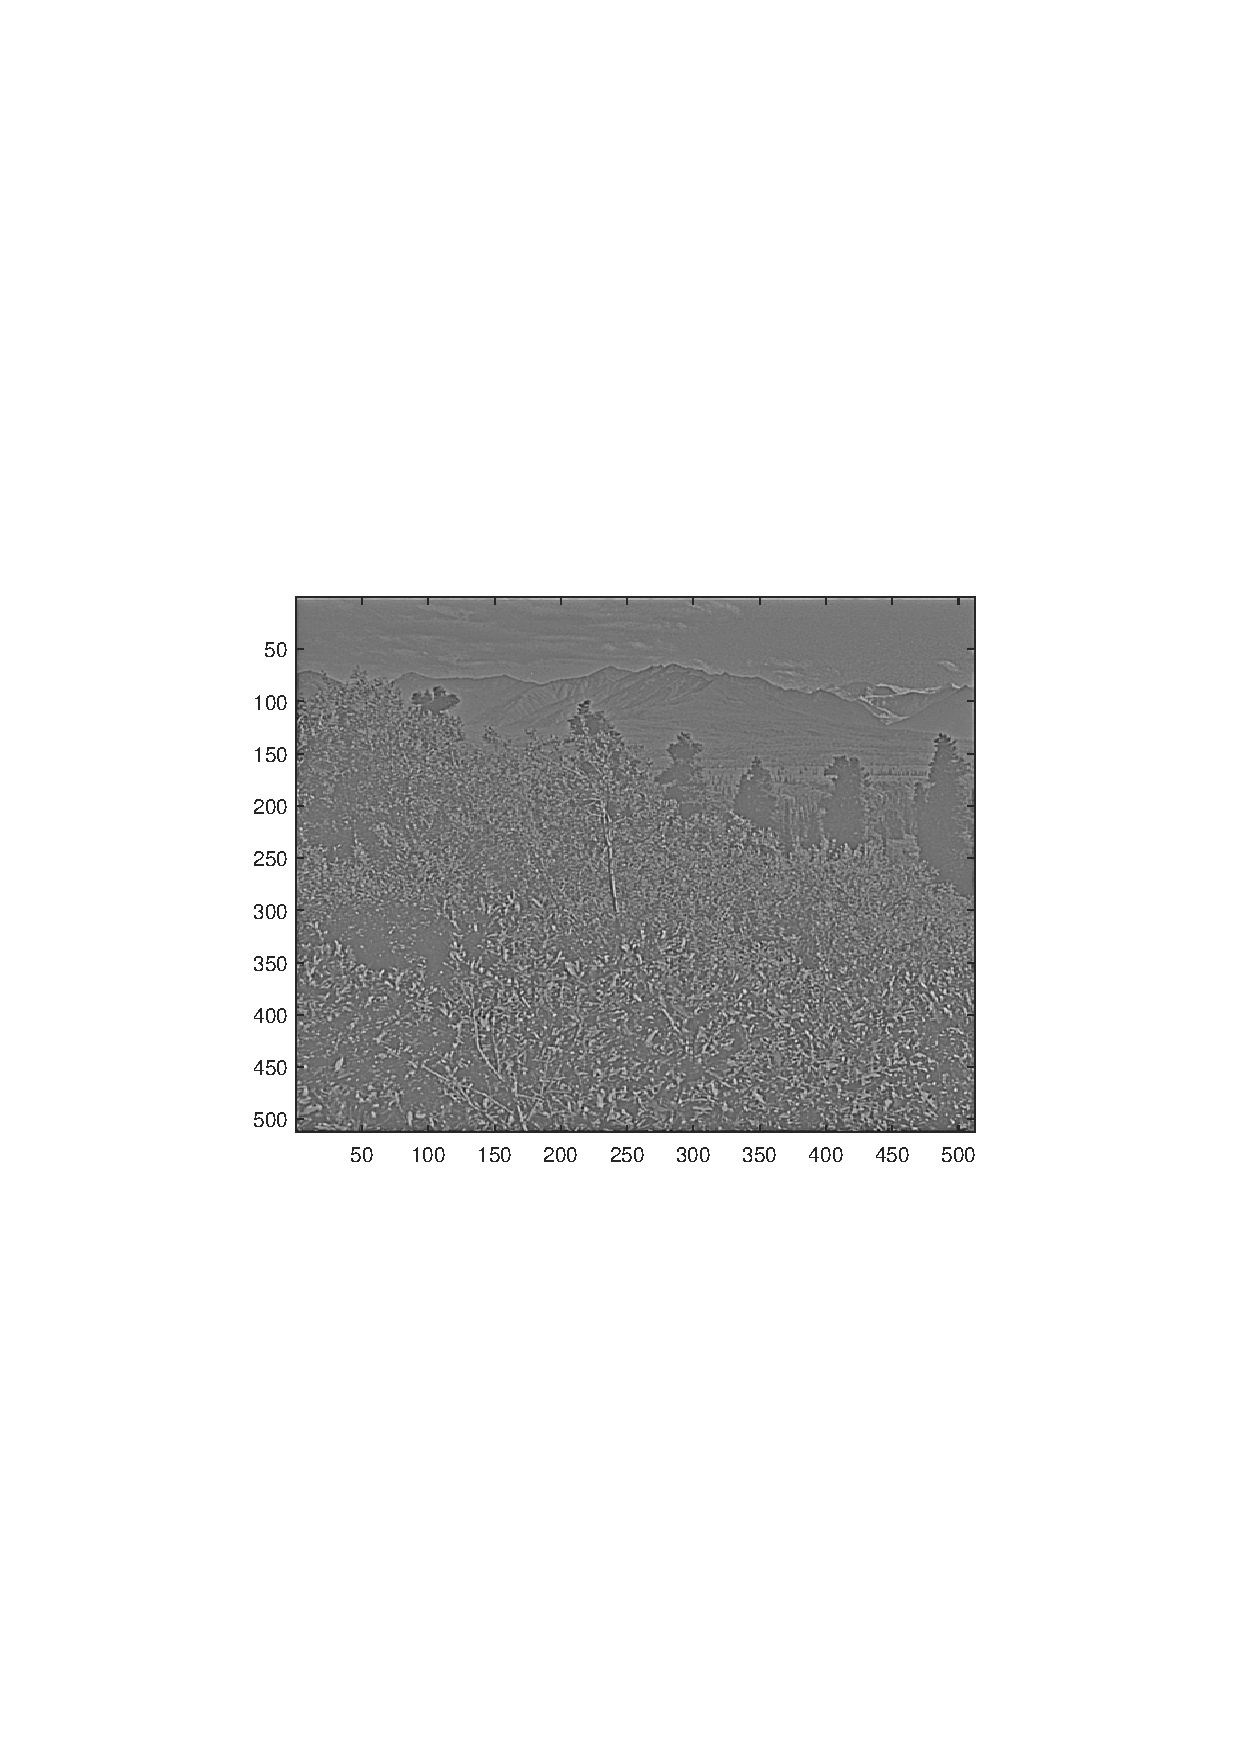
\includegraphics[width=8cm]{fig/INPUT_figure.pdf}
\caption{数据集IMAGES中的一张图片}
\end{figure}

\begin{figure}[H]
\centering
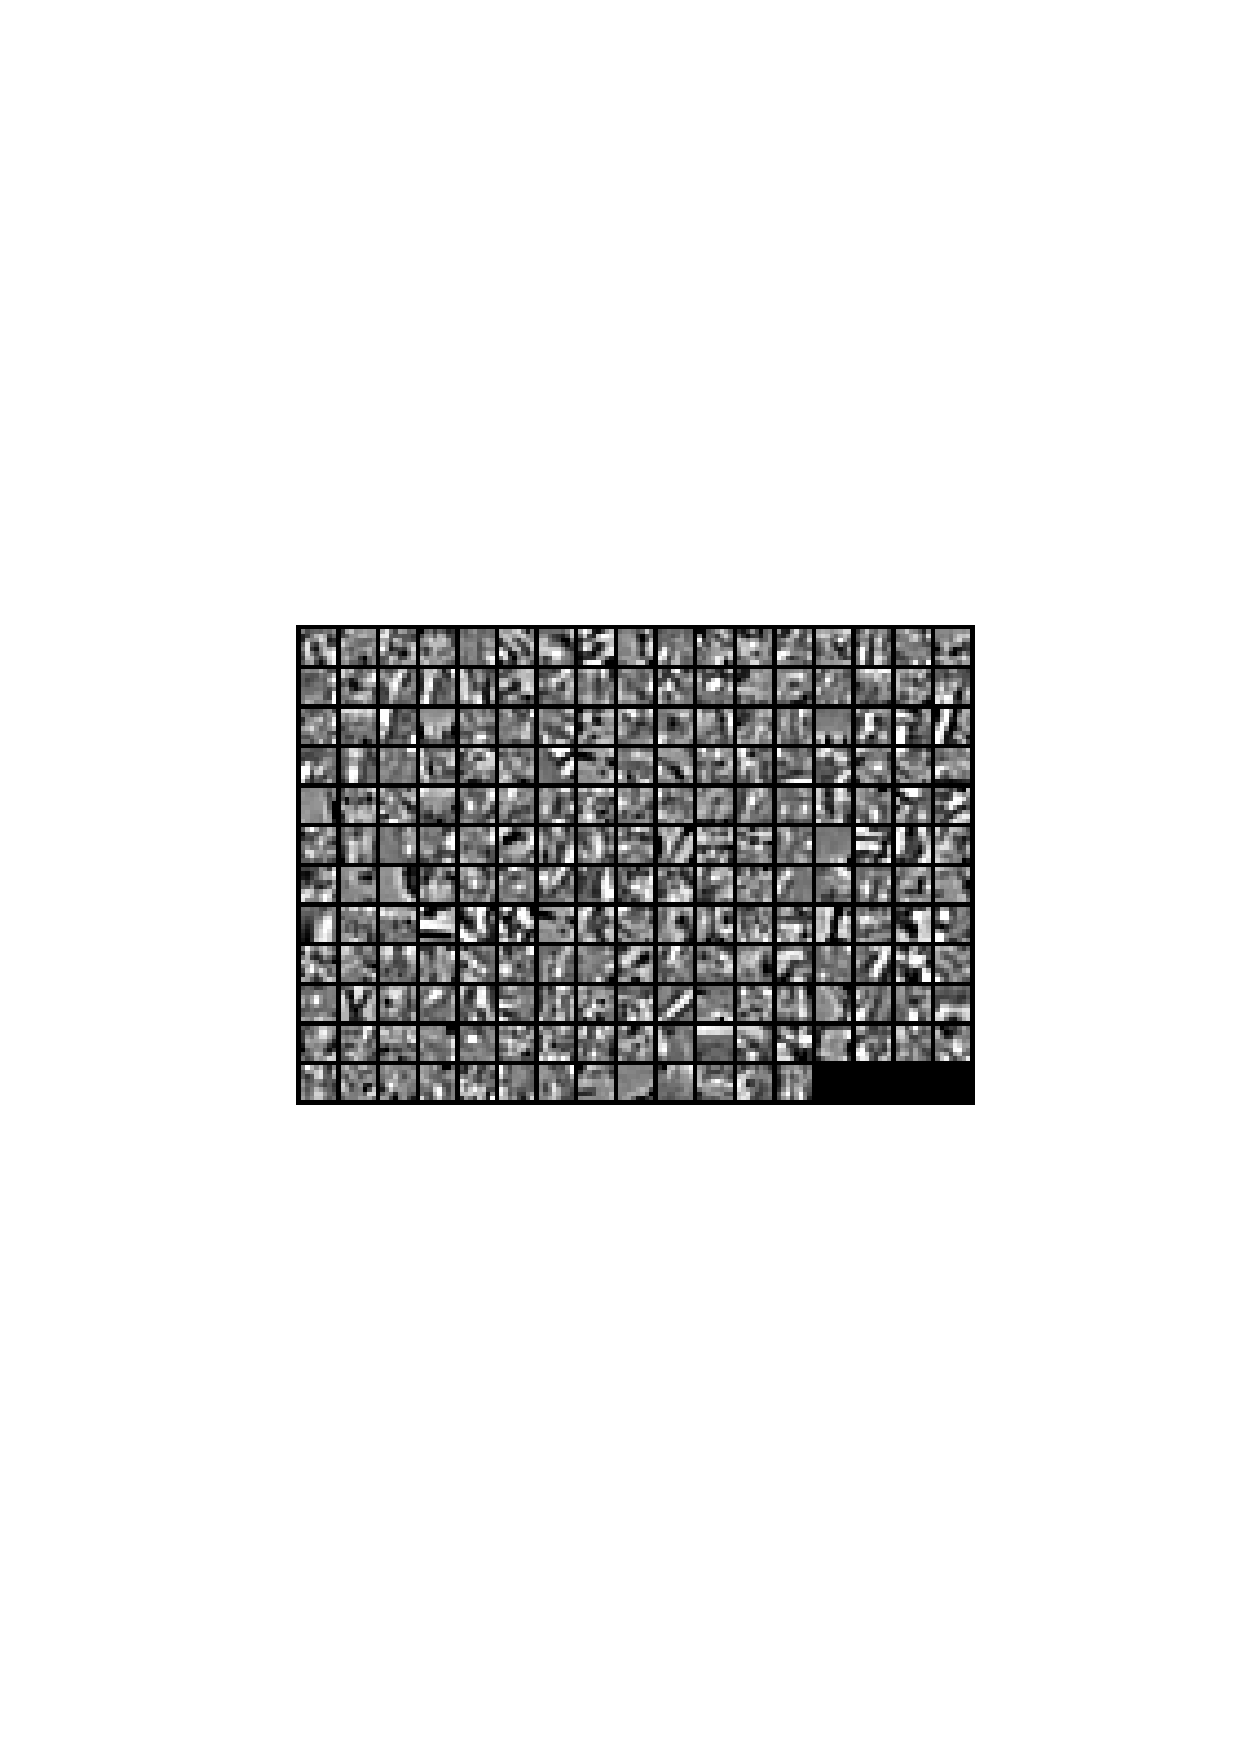
\includegraphics[width=8cm]{fig/sel.pdf}
\caption{随机选出的200张小图片}
\end{figure}


可以看到,这些小格子都是从原图片中分割出来的,
从我们看来,它们杂乱而无规律,但是实际上它们是这张图片的局部缩影,每一张都包含着图片的部分特征。我们将它们作为输入,让神经网络从中学习到特征。

\subsubsection*{神经网络参数}
我们选取神经网络的结构为$[64,25,64]$,稀疏性参数$\rho=0.01$,控制稀疏性惩罚因子的权重 $ \beta =3$,除此之外,我们还加上正则化项,其权重衰减系数$\lambda=0.0001$,

\subsubsection*{训练神经网络}
运行程序 \verb|train.m|就可以开始训练神经网络了。
程序先会显示分割出的训练集图片,不要关闭图片窗口。然后程序会调用封装好的\verb|lbfgs.m|程序进行搜索确定下降方向和步长,并显示显示迭代情况,最后自动输出并保持权值矩阵的图像。

\subsubsection*{权值可视化}
在训练完稀疏自编码器后,我们需要知道这个神经网络到底学到了什么,我们知道,神经网络学习到的东西都存在权值上,而作为自编码器,最重要的权值为$W^{(1)}$,这个权值矩阵是$25\times 64$的,我们将
每一个行向量转化成$8\times8$的矩阵,然后
作为图像输出, 一共25张图像并排输出如下:

\begin{figure}[H]
\centering
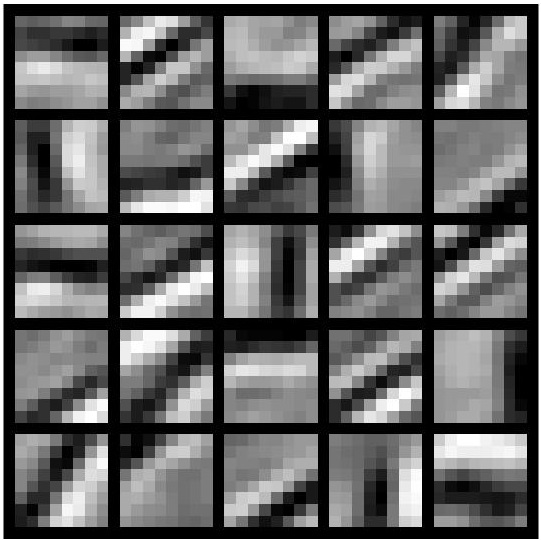
\includegraphics[width=6cm]{fig/s3.jpg}
\caption{权值矩阵的可视化}
\end{figure}

我们可以看到的是,比起之前的输入,这个图像似乎呈现出了
一丝规律性,但这丝规律性又说不清道不明,
这个权值矩阵的图像意味着什么呢?
\subsubsection*{可能的解释}


我们可以从生物学的角度来理解,就像大脑受到某一刺激时某些神经元会兴奋一样,对于输入数据的不同特征,神经网络中会有相应的神经元被激活,如果对于任意特征,都有大量的神经元激活响应,那么神经网络就显得杂乱而低效,所以我们希望单个神经元只对某种特征兴奋。

也就是说,对于由一张图片分割出来的大量小图片,我们希望单个神经元对所有小图片的响应的均值接近0,这就是稀疏性限制,

但是,我们还是需要神经元对于某些图片做出响应,所以我们只需把稀疏性参数$\rho$调小即可。同时,过小的$\rho$会使得神经元被过分压抑,出现这种情况:$W,b$都是负的,且绝对值极大,这就使得对于任意的输入,神经元都不会被激活,为了避免这种情况,所以我们需要加入正则化项,防止极端情况的出现。

那么,对于什么样的输入$\bm{x}$,神经元$i$的激活值最大呢?
我们记$W_i$是由$W^{(2)}_{i1},W^{(2)}_{i1},\cdots,W^{(2)}_{i25}$排成的行向量$[W^{(2)}_{i1},\cdots,W^{(2)}_{i25}]$.

那么
\[a_i^{(2)}(x)=\sigma\left( W_{i}\bm{x}  + b^{(1)}_i \right)\]


给定范数约束$ \|\bm{x}\|^2 = \sum_{i=1}^{64} x_i^2 \leq 1$ ,由于$\sigma(\cdot)$是单调递增的,$W_i,b^{(1)}_i$也是固定值,
在这个条件下,要使$ W_{i}\bm{x}$最大,显然
\[\bm{x}=\dfrac{W_{i}}{ \|W_{i}\|^2}\]

也就是,当输入为权值矩阵$W^{(2)}$第$i$行的行向量时,隐藏层第$i$个神经元的激活值达到最大,或者说,对于这种模式,神经元的响应最剧烈。因此当我们把权值矩阵$W^{(2)}$可视化时,我们看到的就是隐层一个个神经元学习到的模式——不同的隐藏单元学会了在图像的不同位置和方向进行边缘检测。

%显而易见,这些特征对物体识别等计算机视觉任务是十分有用的。若将其用于其他输入域(如音频),该算法也可学到对这些输入域有用的表示或特征。
在这之后,我将抽取的小图片的大小改为$10\times10$,将神经网络的结构改成$[100,100,100]$,最终得到了与原论文类似的图像.

\begin{figure}[H]
\centering
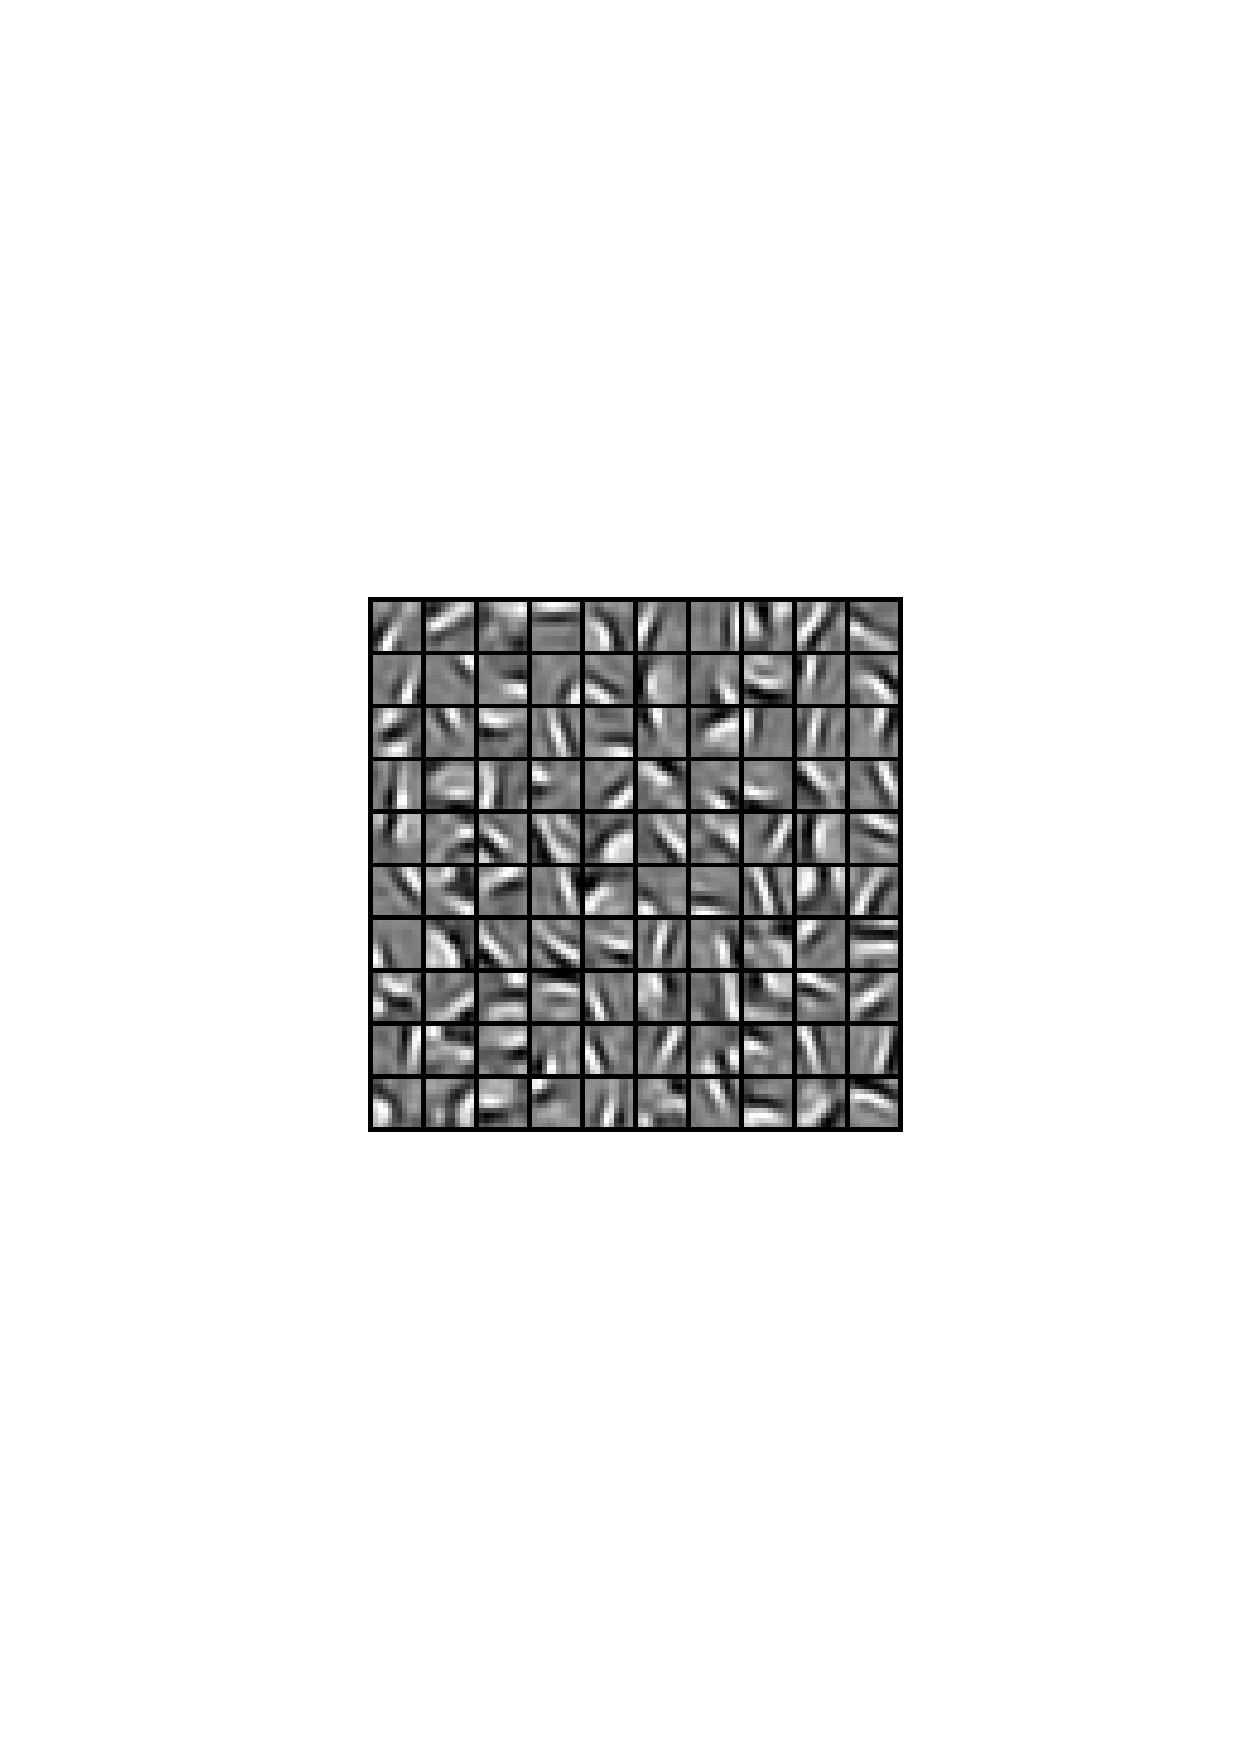
\includegraphics[width=8cm]{fig/s5.pdf}
\caption{新程序学到的特征}
\end{figure}



\subsection{实验2}
实验2是也是基于\href{http://ufldl.stanford.edu/wiki/index.php/UFLDL_Tutorial}{UFLDL Tutorial}的\href{http://ufldl.stanford.edu/wiki/index.php/Exercise:Vectorization}{Exercise:Vectorization}.

从以下两个链接分别下载MNIST手写数字库的训练集图像、训练集分类标签和将这两个文件导入MATLAB的程序:
\begin{itemize}
\item \href{http://yann.lecun.com/exdb/mnist/train-images-idx3-ubyte.gz}{MNIST Dataset (Training Images)}
\item \href{http://yann.lecun.com/exdb/mnist/train-labels-idx1-ubyte.gz}{MNIST Dataset (Training Labels)}
\item \href{http://ufldl.stanford.edu/wiki/resources/mnistHelper.zip}{Support functions for loading MNIST in Matlab}
\end{itemize}

\subsubsection*{文件说明}
\begin{itemize}
 \item \textbf{SAE\_MNIST.m:} 实验的主程序
  \item \textbf{display\_network.m:}用来将数字矩阵转化为图像输出
  \item \textbf{loadMNISTImages.m:}将MNISTI数据集的图像导入MATLAB
 \item \textbf{sparseAutoencoderCost.m:}计算代价函数和梯度
 \item \textbf{lbfgs.m:}可供调用的拟牛顿法程序
\end{itemize}

由于MNIST Dataset中的图像是$28\times28$的,所以需要在原程序上进行参数上的改动,根据Exercise上的说明,将隐藏层神经元的个数设置为196个,那么神经网络的结构为[784,196,784],另外,设置稀疏性参数$\rho=0.1$,控制稀疏性惩罚因子的权重 $ \beta =3$,权重衰减系数$\lambda=0.003$,由于计算量过大,所以只选取5000张图片作为训练集,
之后启动主程序\verb|SAE_MNIST.m|开始训练神经网络,在400次迭代后输出权值矩阵图像。

\begin{figure}[H]
\centering
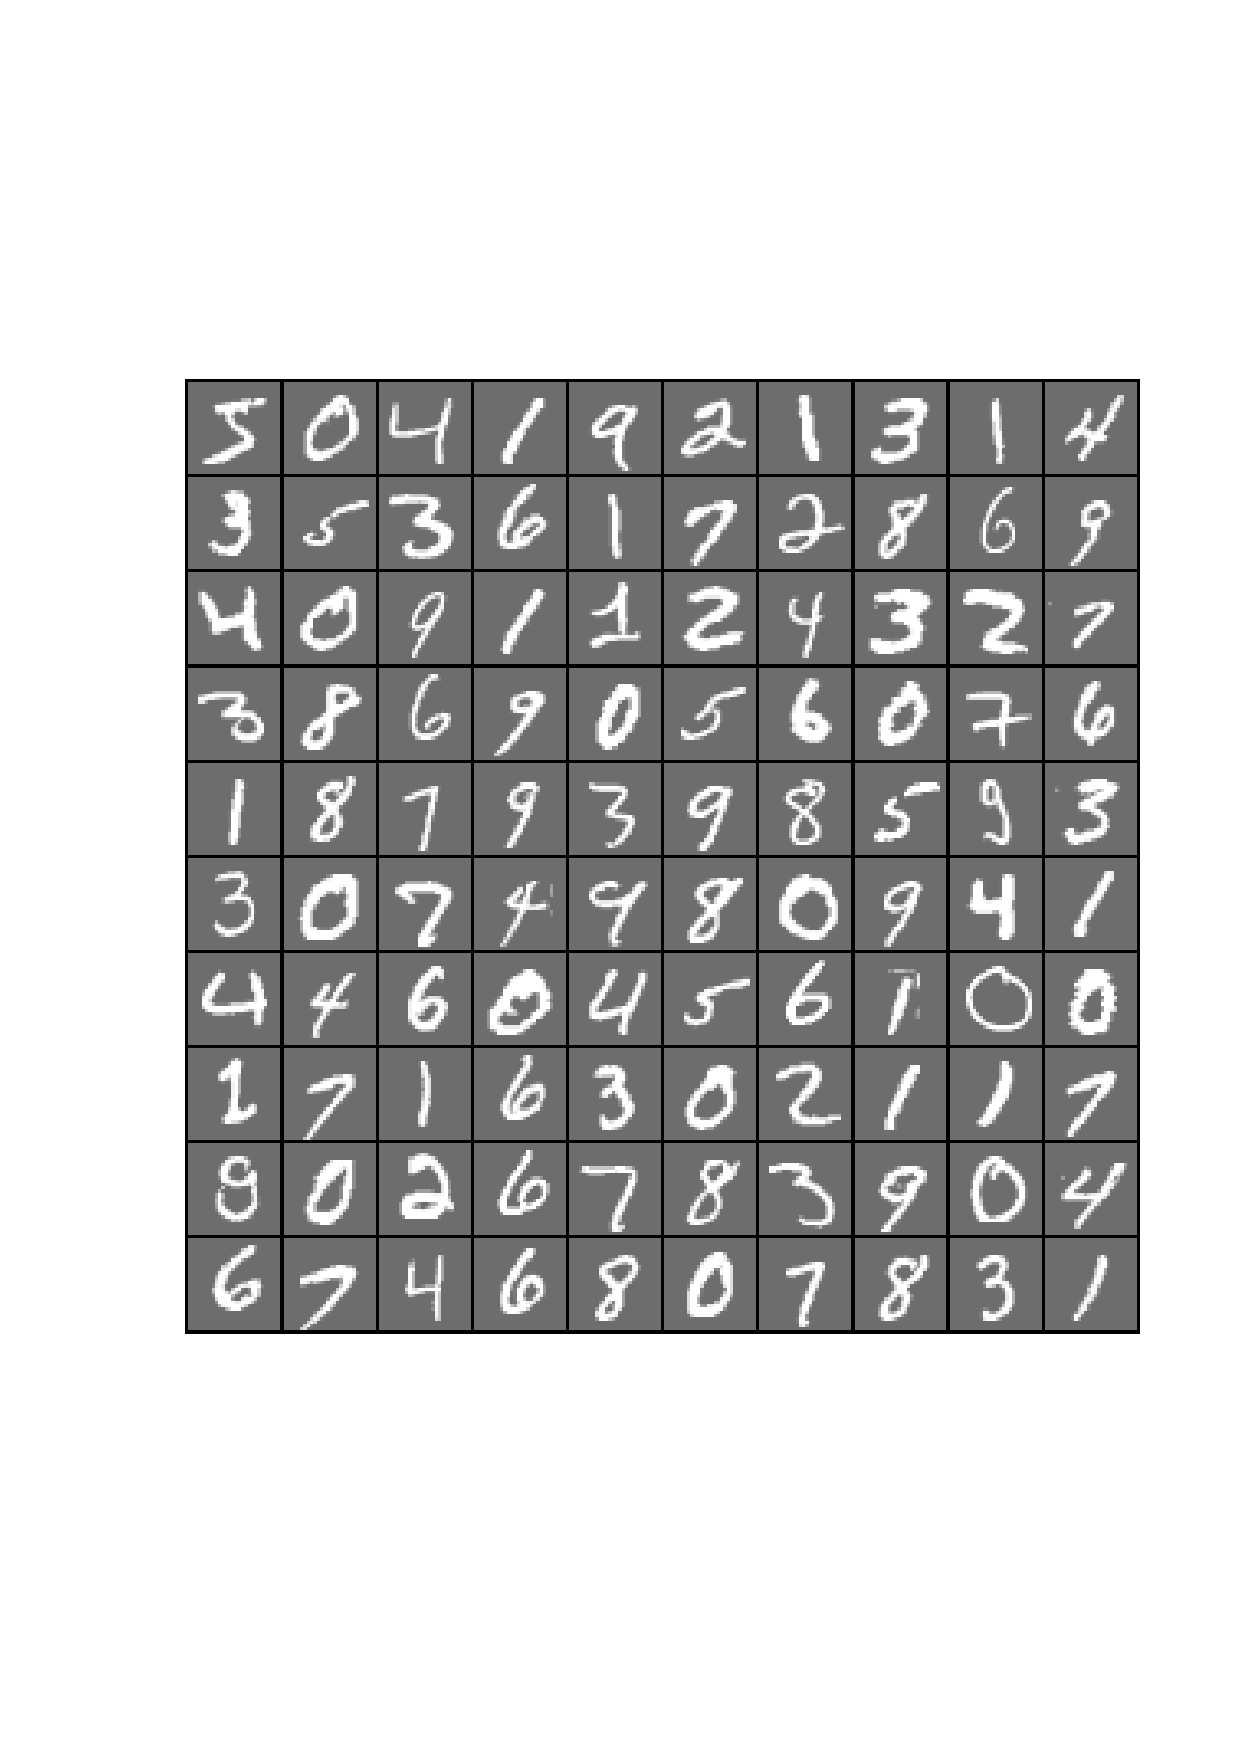
\includegraphics[width=7cm]{fig/MNISTI_input.pdf}
\caption{MNISTI手写数字}
\end{figure}

\begin{figure}[H]
\centering
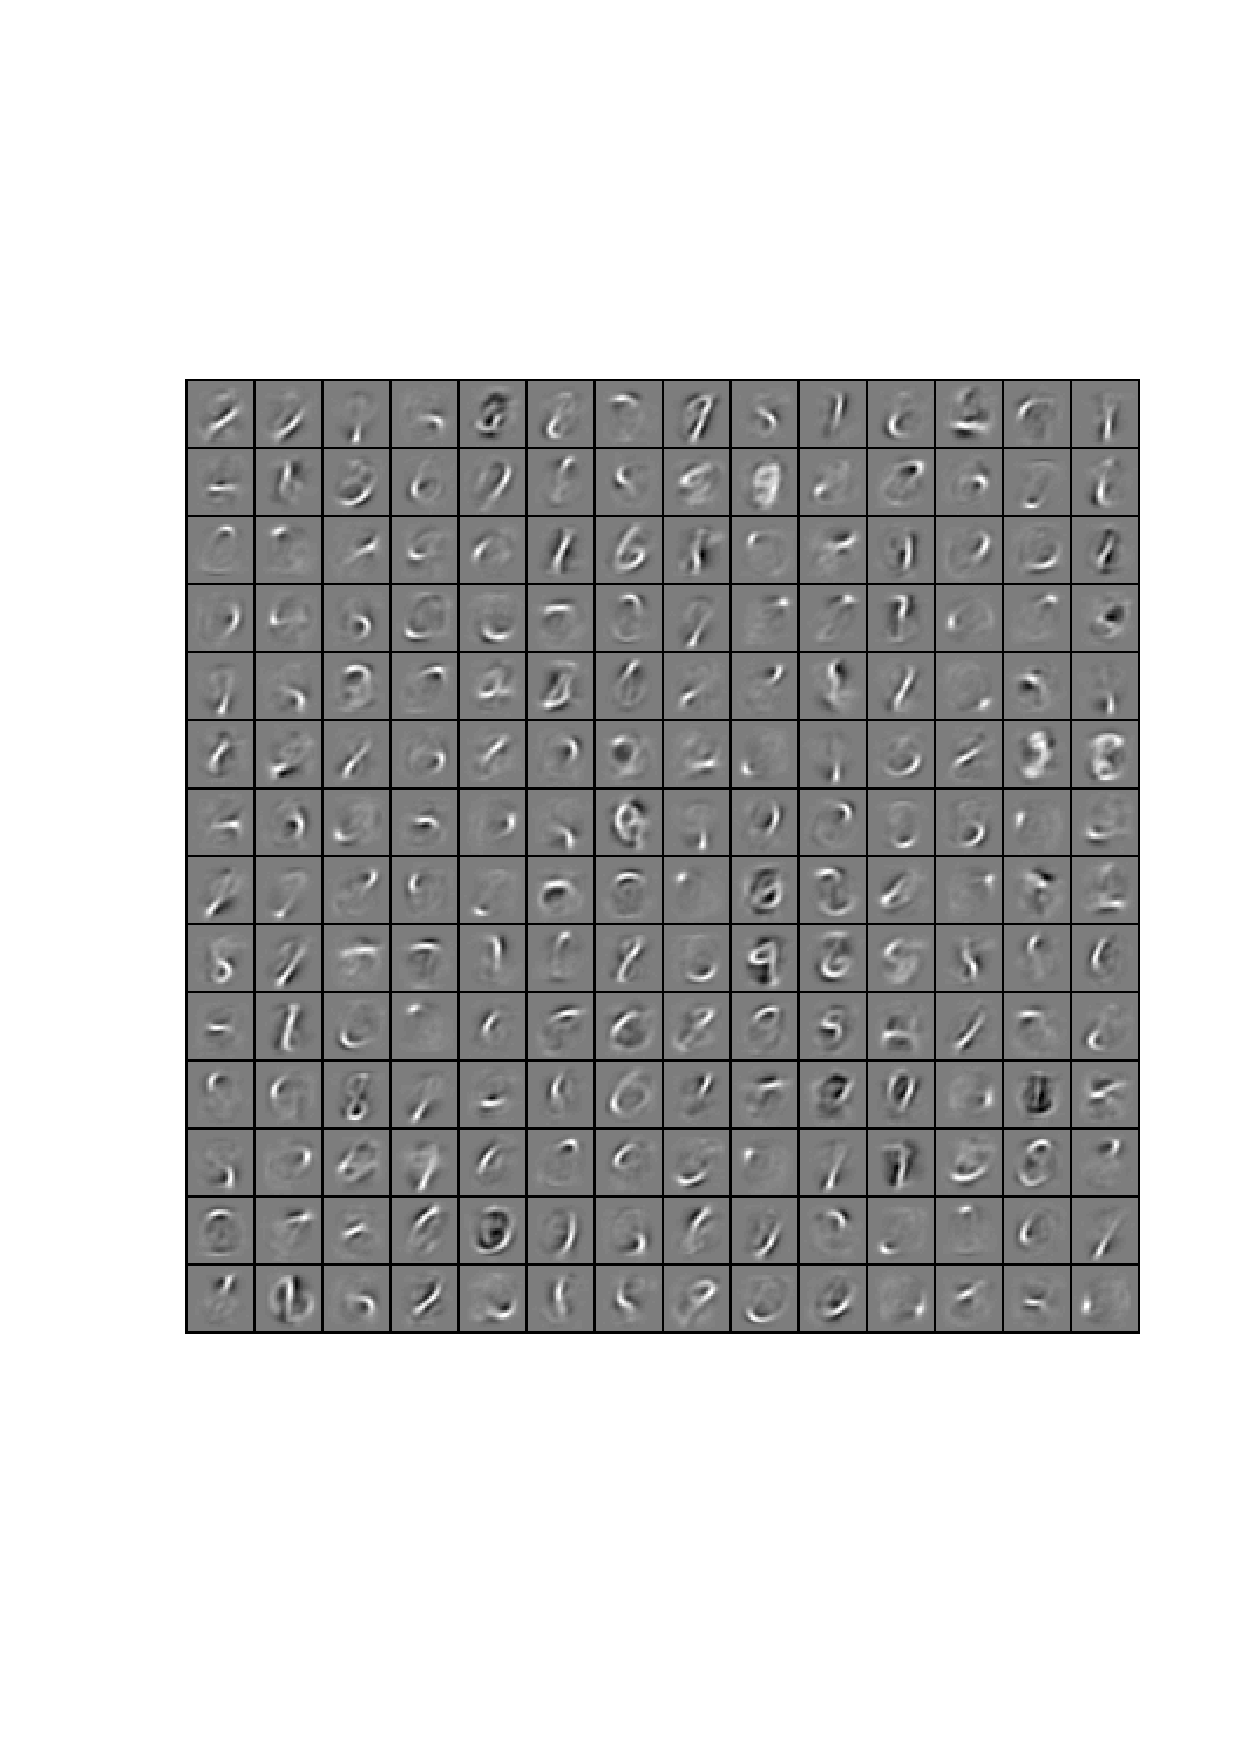
\includegraphics[width=10cm]{fig/MNISTI_output.pdf}
\caption{学习到的模式}
\end{figure}

观察图像,总体上来说,神经网络还是学习到了手写数字的特征——有的神经元学到了点、横、竖、撇、捺等,但也能看出,有的神经元学习得并不彻底,隐约还能看到原来数字的轮廓。

\textbf{总结:}这些特征对物体识别等计算机视觉任务是十分有效的。若将其用于其他输入域(如音频),该算法也可学到对这些输入域有用的表示或特征。
\end{document}